\documentclass{beamer}

\usepackage{amsmath, amssymb}
\usepackage{tikz-cd}
\usepackage{xcolor}
\usepackage{graphicx}

\title{MAT414 - Modern Algebra}
\author{\textbf{Miraj Samarakkody}}
\institute{Tougaloo College}
\date{03/31/2025}

\begin{document}

\begin{frame}
    \titlepage
\end{frame}



    \begin{frame}{}
    \begin{center}
        \Huge{Fundamental Theorem of Cyclic Groups}
    \end{center}
    \end{frame}

    \begin{frame}{Theorem 4.3}
    \begin{block}{Fundamental Theorem of Cyclic Group}
        Every subgroup of a cyclic group is cyclic. Moreover, if \(|\langle a \rangle|=n\), then  the order of any subgroup of \(\langle a\rangle\) is a divisor of n; and, for each positive divisor \(k\) of \(n\), the group \(\langle a\rangle\) has exactly one subgroup of order \(k-\)namely, \(\langle a^{n/k}\rangle\). 
    \end{block}
    \end{frame}

  

    \begin{frame}
        \frametitle{Corollary}
        \begin{block}{Subgroups of \(\mathbb{Z}_n\)}
        For each positive divisor \(k\) of \(n\), the set \(\langle n/k\rangle\) is the unique subgroup of \(\mathbb{Z}_n\) of order \(k\); moreover, these are the only subgroups of \(\mathbb{Z}_n\).    
        \end{block}
    \end{frame}



\begin{frame}
    \frametitle{Example 8}
Find the generators of the subgroup of order 9 in \(\mathbb{Z}_{36}\). 
    

\end{frame}


\begin{frame}
    \frametitle{Euler Phi Function}
Let \(\phi(1)=1\), and for any integer \(n>1\), let \(\phi(n)\) denote the number of positive integers less than \(n\) and relatively prime to \(n\). 

\begin{block}{Example} Write each \(\phi(n)\) for \(n \in \{1,2, \dots, 12\}\)
    
\end{block}


\begin{block}{Some Properties}
    \begin{itemize}
        \item For any prime \(p\), \(\phi(p^n)=p^n-p^{n-1}\)
        \item For relatively prime \(m\) and \(n\), \(\phi(mn)=\phi(m)\phi(n)\)
    \end{itemize}
\end{block}

    

\end{frame}

\begin{frame}
    \frametitle{Theorem 4.4}

    \begin{block}{Number of Elements of Each Order in a Cyclic Group}
        If \(d\) is a positive divisor of \(n\), the number of elements of order \(d\) in a cyclic group of order \(n\) is \(\phi(d)\).         
    \end{block}\pause

\end{frame}

\begin{frame}
    \frametitle{Corollary}

    \begin{block}{Number of Elements of Order \(d\) in a Finite Group}  
        In a finite group, the number of elements of order \(d\) is a multiple of \(\phi(d)\). 
    \end{block}

\end{frame}

\begin{frame}
    \frametitle{Subgroup Lattice }

    The  relationship among the various subgroups of a group can be illustrated with a subgroup lattice of the group. This is a diagram that includes all the subgroups of the groups of the group and connects a subgroup \(H\) at one level to a subgroup \(K\) at a higher level with a sequence of line segments if and only if \(H\) is a proper subgroup of \(K\). 

    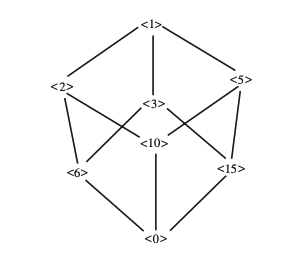
\includegraphics[scale=0.5]{Figures/fig_1.png}

\end{frame}



\end{document}